\subsection{Introduction}

\begin{frame}[t]
    \Title{White-box Cryptography}

    \nocitepartiii{mybibWhitebox}
    \bibliographystylepartiii{unsrt}
    
    \Block{3cm,3.5cm}{10cm}{
        \bibliographypartiii{mybiblio.bib}
    }
\end{frame}

\begin{frame}
\Title{White-box model}
\Block{10.75cm,3.5cm}{5cm}{
	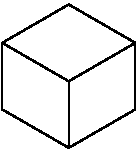
\includegraphics[height=5cm]{whitebox-simple.pdf}
}
\pause
\begin{itemize}
    \item implementation is fully \alert{available} to an adversary
    \item secret key should be \alert{unextractable}
    \item {\bf extra}: one-wayness, incompressibility, traitor traceability, ...
\end{itemize}
\vspace{1cm}
\pause
\begin{itemize}
    \item The most {\bf challenging} direction (this work): \\
          white-box implementations of \\
          \alert{existing} symmetric primitives, \\
          e.g. the AES block cipher
    % \item ``Cryptographic \textcolor{blue}{obfuscation}''
\end{itemize}
\end{frame}


\begin{frame}[t]
    \CreditsTikz{}
    \Title{Example: \textcolor{green!50!black}{Secure} White-box}
    
    \only<1>{
    \vspace{0.5cm}
    \Center{
        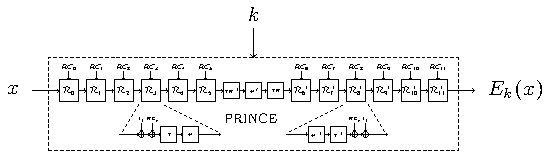
\includegraphics[height=4cm]{figures/whitebox.pdf}
    }}
    
    \only<2->{
    \Center{
        \begin{tabular}{|c|c|}
\hline
$x$ & $E(x)$ \\
\hline
\texttt{\footnotesize{0000000000000000}} & \texttt{\footnotesize{9333dd078833edd3}} \\
\texttt{\footnotesize{0000000000000001}} & \texttt{\footnotesize{7072b89243c84359}} \\
\texttt{\footnotesize{0000000000000002}} & \texttt{\footnotesize{7838040f2b7f9af6}} \\
\texttt{\footnotesize{0000000000000003}} & \texttt{\footnotesize{0b502e4231f42da3}} \\
\texttt{\footnotesize{0000000000000004}} & \texttt{\footnotesize{c39ea8c9434252aa}} \\
\hline
\multicolumn{2}{|c|}{\ldots} \\
\hline
\texttt{\footnotesize{fffffffffffffffb}} & \texttt{\footnotesize{8f1a82bc7af09497}} \\
\texttt{\footnotesize{fffffffffffffffc}} & \texttt{\footnotesize{9aaf33009a8e9a2f}} \\
\texttt{\footnotesize{fffffffffffffffd}} & \texttt{\footnotesize{5cd335922f9f0236}} \\
\texttt{\footnotesize{fffffffffffffffe}} & \texttt{\footnotesize{39d0e8b9a0eded09}} \\
\texttt{\footnotesize{ffffffffffffffff}} & \texttt{\footnotesize{daf2ced4ab8fc658}} \\
\hline
        \end{tabular}
    }
    }
    
    \only<3>{
    \Center{
        \Large \alert{Impractical! $128$ exbibytes for a 64-bit cipher!}
    }
    }
\end{frame}


\begin{frame}[t]
\Title{White-box: Industry vs Academia}

\begin{columns}[c]
  \column{0.1\linewidth}{}
  \column{0.35\linewidth}{
    \Center{
\includegraphics[height=2cm]{figures/industry.png}}
  }
  \column{0.35\linewidth}{
    \Center{
\includegraphics[height=2cm]{figures/academia.png}}
  }
  \column{0.1\linewidth}{}
\end{columns}  
\begin{columns}
  \pause
  \column{0.05\linewidth}{}
  \column{0.4\linewidth}{
    \CenterBlock{5.5cm}{
	\begin{itemize}	
        \item WB has many applications
        \item strong need for \emph{efficient} WB
		\item industry {\bf does} WB: \\
		      \alert{hidden designs}
	\end{itemize}
	}
  }
  \pause
  \column{0.4\linewidth}{
    \CenterBlock{6cm}{
	\begin{itemize}	
		\item {\bf theory}: approaches using iO/FE, currently \emph{impractical}
		\item {\bf practical WB-AES}: \\
              few attempts (2002-2017), \\
              \alert{all broken}
        \item powerful DCA attack \\
              (CHES 2016)
	\end{itemize}
	}
  }
  \column{0.05\linewidth}{}
\end{columns}
\end{frame}

\begin{frame}
\Title{White-Box: Differential Computation Analysis (DCA)}

\center{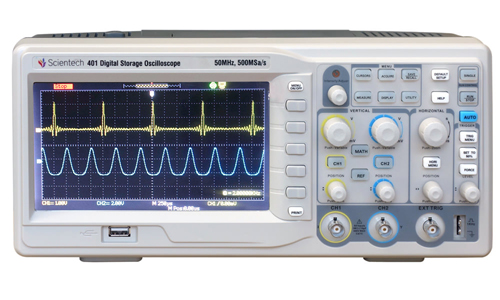
\includegraphics[height=3cm]{figures/oscilloscope.jpg}}
\CenterBlock{12cm}{
\vspace{0.25cm}
\begin{itemize}	
	\item {\bf DCA} = {\bf Differential Power Analysis (DPA)} \\
	      applied to white-box implementations
	\item Most of the implementations \alert{broken automatically}
	\pause
	\item Side-channel protection: {\bf masking schemes}
\end{itemize}
}
\pause
\center{
    \emph{this work}: \\
    {\color{PineGreen}Can we apply the masking protection for white-box impl.?} 
}
\end{frame}

\begin{frame}
\Title{General Setting}    

\CenterBlock{12cm}{
\vspace{0.5cm}
\begin{itemize}
    \item Boolean {\bf circuits}
    \item {\bf obfuscated} reference implementation
    \pause
    \item {\bf predictable values}: computations from ref. impl., e.g.
        $$s = Bit_1(SBox(pt_1\oplus k_1))$$
    \pause
    \item {\bf masking}: $\exists v_1,\ldots,v_t$ nodes (\emph{shares}), $f: \field{t}\to \field{}$ s.t. for any encryption
        $$f(v_1,\ldots, v_t)=s$$
\end{itemize}
}
\end{frame}

\begin{frame}
\Title{Masking Schemes}

\CenterBlock{12cm}{
\vspace{0.5cm}
\begin{itemize}
    \item {\bf Example~~} Boolean masking: linear decoder $f=\bigoplus_i v_i$
    \item {\bf Example~~} FHE: complex non-linear decoder $f$
    \pause
    \item Aim for \textcolor{green!40!black}{efficient} schemes: relatively small $t$ (number of shares)
\end{itemize}
}

\pause

\center{
    $\Rightarrow$ \alert{can be secure only if \\
    the locations of the shares in the circuit are unknown!}
}

\center{\emph{this work}: exploring this possibility}

\end{frame}